\begin{boxB}
    بیایید الگوریتم‌های AES (استاندارد رمزگذاری پیشرفته) و Twofish را بر اساس اندازه کلید، اندازه بلوک و سطوح امنیتی مقایسه کنیم.
    
1. اندازه کلید:
    - AES: 
    
    AES اندازه های کلیدی 128، 192 و 256 بیت را پشتیبانی می کند.
    
    - Twofish:
    
    Twofish از اندازه های کلیدی 128، 192 و 256 بیتی پشتیبانی می کند.

2. اندازه بلوک:
    - AES:
    AES دارای اندازه بلوک ثابت 128 بیت (16 بایت) است.
    
    - Twofish:
    Twofish دارای اندازه بلوک متغیر است که می تواند 128، 192 یا 256 بیت (16، 24، یا 32 بایت) باشد.


3. سطح امنیتی:
    - AES:
    
    AES به طور گسترده توسط رمزنگاران در سراسر جهان مورد مطالعه و تجزیه و تحلیل قرار گرفته است. به طور گسترده ای امن در نظر گرفته می شود و استاندارد رمزگذاری است که توسط دولت ها و سازمان ها در سطح جهانی استفاده می شود. AES-128 از نظر محاسباتی در برابر حملات brute-force ایمن در نظر گرفته می شود.
    
    - Twofish:
    
    Twofish نیز مورد تجزیه و تحلیل کامل قرار گرفته و امن محسوب می شود. با این حال، در مقایسه با AES مورد بررسی گسترده کمتری قرار گرفته است. دو ماهی به طور کلی در نظر گرفته می شود که سطح بالایی از امنیت را ارائه می دهد، قابل مقایسه با AES.


4. عملکرد:
    - AES: 
    
    AES به دلیل کارایی خود در اجرای نرم افزار و سخت افزار شناخته شده است. این بسیار بهینه شده است و به طور گسترده توسط پلتفرم ها و کتابخانه های مختلف پشتیبانی می شود.
    
    - Twofish:
    
    Twofish نیز کارآمد است اما ممکن است در سناریوهای خاص عملکرد کمی در مقایسه با AES داشته باشد.



5. ساختار الگوریتم:
    - AES:
    
    AES یک الگوریتم کلید متقارن مبتنی بر ساختار شبکه جایگزینی-جایگزینی (SPN) است. این شامل چندین دور عملیات تعویض بایت، جابجایی و اختلاط است.
    
    - Twofish:
    
    Twofish یک الگوریتم کلید متقارن بر اساس ساختار شبکه Feistel است. از ترکیبی از جعبه های S وابسته به کلید، جایگشت های وابسته به کلید و عملیات اختلاط استفاده می کند.


6. پذیرش الگوریتم:
    - AES:
    
    AES به عنوان الگوریتم رمزگذاری استاندارد توسط سازمان های مختلف از جمله دولت ایالات متحده پذیرفته شده است. به طور گسترده در برنامه ها و پروتکل هایی که نیاز به رمزگذاری ایمن دارند استفاده می شود.
    
    - Twofish:
    
    Twofish در مرحله انتخاب AES فینالیست شده است اما به عنوان استاندارد انتخاب نشده است. با این حال، هنوز به عنوان یک جایگزین قوی در نظر گرفته می شود و در برنامه های مختلف و محصولات امنیتی مورد استفاده قرار گرفته است.


هر دو AES و Twofish الگوریتم های رمزگذاری ایمن هستند که برای اکثر برنامه ها مناسب هستند. AES به طور گسترده‌تری پذیرفته شده و استاندارد شده است، در حالی که Twofish یک گزینه جایگزین با ویژگی‌های امنیتی مشابه ارائه می‌کند. انتخاب بین این دو به عواملی مانند الزامات سازگاری، در دسترس بودن الگوریتم و نیازهای امنیتی خاص بستگی دارد. هنگام انتخاب یک الگوریتم رمزگذاری، توجه به اکوسیستم رمزنگاری اطراف، پشتیبانی پلت فرم، و الزامات مورد استفاده فردی مهم است.
\end{boxB}

\begin{figure}
    \centering
    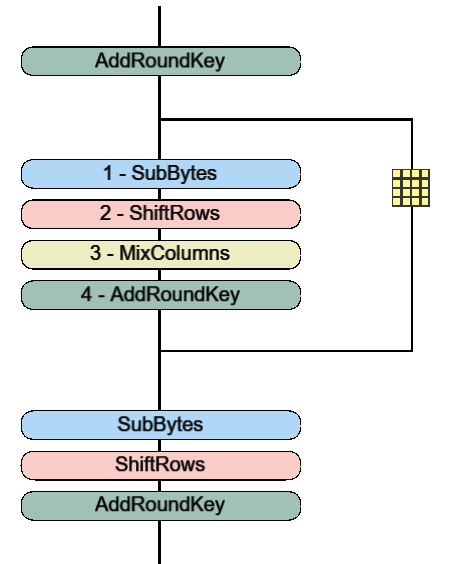
\includegraphics{Final/images/AES.png}
    \caption{AES Algorithm}
    \label{fig:enter-label}
\end{figure}